\section{Modelos lineales}

Los modelos lineales son un tipo de modelo matemático que utilizan una función lineal para describir la relación entre dos o más variables. Estos modelos son ampliamente utilizados en muchas áreas, como la economía, la ingeniería, la física y la psicología, debido a su simplicidad y facilidad de interpretación. Además, son útiles para hacer predicciones sobre el comportamiento de un sistema en el futuro. 
\newline

Un modelo lineal se compone de una ecuación matemática que describe la relación entre las variables independientes y la variable dependiente. Es importante tener en cuenta que los modelos lineales tienen algunas limitaciones, como la supuesta linealidad de la relación entre las variables y la supuesta independencia y homogeneidad de los errores. Estas limitaciones deben tenerse en cuenta al utilizar este tipo de modelos.

\subsection{Linear Regression}

El \cite{Sklearn Linear Regression} es un modelo lineal que permite ajustar a un conjunto de datos y utilizarlo para hacer predicciones. Este modelo se basa en la minimización de la suma de los cuadrados de los residuos entre las predicciones del modelo y los datos observados, y se puede utilizar tanto para resolver problemas de regresión como de clasificación binaria. En este modelo no se pueden modificar los parametros, por lo que la experimentación es bastante sencilla. Se ha entrenado el modelo con los datos estandarizados y con la resta de las variables objetivo, hecho que nos ha permitido obtener los siguientes resultados.

\begin{figure}[H]
    \centering
    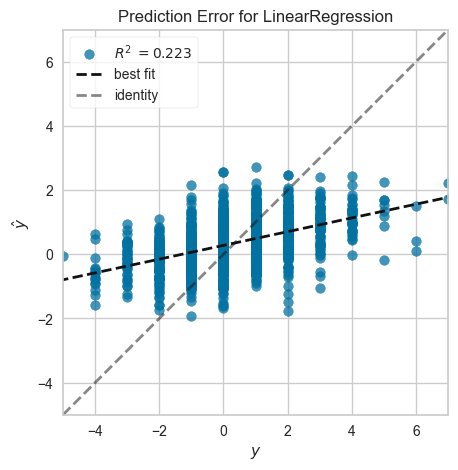
\includegraphics[width=\smallSize]{images/linearModelLinearRegression.png}
    \caption{Linear Regression: Prediccion del error}
    \label{Modelos-Lineales-Linear-Regression-Prediccion-Error}
\end{figure}

En la Figura \ref{Modelos-Lineales-Linear-Regression-Prediccion-Error} podemos ver como los resultados obtenidos no son demasiado satisfactorios. Esta conclusion se puede obtener tanto graficamente como analiticamente, consultando el valor $R^2$ que equivale a $0.223$. 
\newline

Además, se realizará con todos los modelos es el calculo del tiempo medio de entrenamiento, en este caso, el modelo de regresión lineal tiene un tiempo de entrenamiento medio de $0.013$ segundos. Por otra parte, al ejecutar la Validación cruzada al modelo entrenado se han obtenido, de media, un valor de $0.216$. Si nos fijamos en los valores obtenidos por cada uno de los pliegues que se ha realizado al conjunto de datos encontramos en el Cuadro \ref{Modelos-Lineales-Linear-Regression-Validacion-Cruzada}.

\begin{table}[h]
    \centering
    \begin{tabular}{lccccc}
        \textbf{Pliegue} & 1 & 2 & 3 & 4 & 5 \\
        \textbf{Resultado} & 0.25609482 & 0.1231758 & 0.25783003 & 0.16857474 & 0.27594974
    \end{tabular}
    \caption{Linear Regression: Resultados Validación Cruzada}
    \label{Modelos-Lineales-Linear-Regression-Validacion-Cruzada}
\end{table}

\subsection{Ridge Regression}

La \cite{Sklearn Ridge} es una variante de la \cite{Sklearn Linear Regression} que se utiliza para controlar el sobreajuste. A diferencia de la Regresión Lineal, que solo minimiza la suma de los cuadrados de los residuos entre las predicciones del modelo y los datos observados, la Ridge Regression también agrega una penalidad por la magnitud de los coeficientes del modelo. Esta penalidad se controla mediante el parámetro alpha, que determina qué tanto se penalizan los coeficientes.
\newline

La Ridge Regression es útil en situaciones en las que el conjunto de datos tiene una alta dimensionalidad y existe el riesgo de que el modelo se sobreajuste. Al penalizar los coeficientes del modelo, la Ridge Regression puede ayudar a evitar el sobreajuste y mejorar la generalización del modelo a datos nuevos.
\newline

En este caso, se ha decidido empezar la experimentación encontrando el valor óptimo para el parámetro alpha. Se ha entrenado el modelo por una lista finita de valores comprendidos entre 0, que anula los pesos y por lo tanto es equivalente a la Linear Regression, y 10. Después de comprovar los resultados de la validación cruzada y el valor de $R^2$, se ha podido observar como el resultado es el mismo por todos los valores possibles de alpha, hecho que nos lleva a pensar que no existe sobreajuste. 
\newline

\begin{figure}[H]
    \centering
    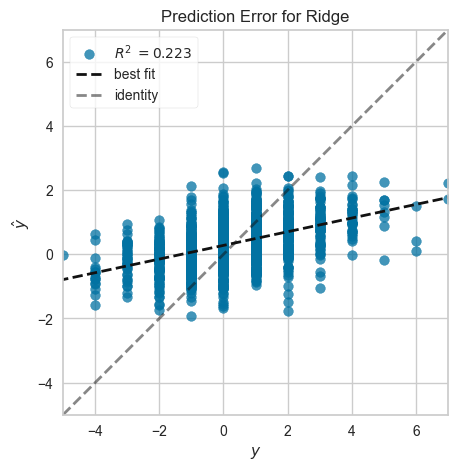
\includegraphics[width=\smallSize]{images/linearModelRidge.png}
    \caption{Ridge Regression: Prediccion del error}
    \label{Modelos-Lineales-Ridge-Prediccion-Error}
\end{figure}

De la misma forma que en el modelo de Regresión Lineal, en la Figura \ref{Modelos-Lineales-Ridge-Prediccion-Error} podemos ver como los resultados obtenidos no son demasiado satisfactorios. El valor de $R^2$, es el mismo que en la Regresión Lineal $0.223$, pero el valor de la validación cruzada ha mejorado levemente. En este caso, la media de las validaciónes cruzada es $0.218$. Y si queremos fijarnos en los valores individuales de cada validación, lo podemos encontrar en el Cuadro \ref{Modelos-Lineales-Ridge-Validacion-Cruzada}.

\begin{table}[h]
    \centering
    \begin{tabular}{lccccc}
        \textbf{Pliegue} & 1 & 2 & 3 & 4 & 5 \\
        \textbf{Resultado} & 0.25630708 & 0.12472019 & 0.25798172 & 0.17091906 & 0.28008048
    \end{tabular}
    \caption{Ridge Regression: Resultados Validación Cruzada}
    \label{Modelos-Lineales-Ridge-Validacion-Cruzada}
\end{table}

Para acabar, se ha visto que en este caso, el tiempo de entrenamiento es inferior al de la regression lineal, obteniendo un valor cercano a $0.002$ segundos de media. 
\subsection{KNeighbors Regressor}
\subsection{Resultados}

A continuación en el Cuadro \ref{Modelos-No-Lineales-Resultados} encontramos de forma sintetica los resultados de cada modelo, donde se puede comparar de forma analitica los distintos modelos, teniendo en cuenta tanto los resultados de las validaciones como el tiempo de entrenamiento necesario. 

\begin{table}[h]
    \centering
    \begin{tabular}{lccc}
                                        & \textbf{$R^2$} & \textbf{Validación Cruzada}  & \textbf{Tiempo de Entrenamiento} \\
        \textbf{Random Forest}          &  0.2031   &        0.2025     & 1.3928 \\
        \textbf{SVM Kernel RBF}         &  0.2889   &        0.2866     & 0.8234 \\
        \textbf{MLP}                    &  0.2282	&        0.2115     & 1.5283
    \end{tabular}
    \caption{Resultados Modelos No Lineales}
    \label{Modelos-No-Lineales-Resultados}
\end{table}

\newpage